\subsection{Modelado de sistemas}
\label{sec:modelado_de_sistemas}
El modelado de sistemas y de relaciones entre variables es una tarea fundamental en múltiples áreas de la ingeniería y la ciencia. Un sistema puede definirse como una relación funcional entre variables de entrada $x$ y salida $y$, donde la salida es una función de las entradas $y = f(x)$ como se muestra en la \reffig{system}.

\begin{figure}[H]
    \centering
    \begin{tikzpicture}
        \node (input) at (0, 0) [] {$x$};
        \node[rectangle, draw, minimum width=2cm, minimum height=1cm, right=of input] (system) {$f$};
        \node (output) [right=of system] {$y$};
        \draw[-stealth] (input) -- (system);
        \draw[-stealth] (system) -- (output);
    \end{tikzpicture}
    \caption{Sistema a modelar.}
    \label{fig:system}
\end{figure}

En el caso general, la salida observada $y$ puede estar afectada por ruido, lo que dificulta la tarea de modelado, ya que agrega incertidumbre a la relación entre las variables de entrada y salida \cite{Bishop2006}.

    \begin{figure}[H]
        \centering
        \begin{tikzpicture}
            \node (input) at (0, 0) [] {$x$};
            \node[rectangle, draw, minimum width=2cm, minimum height=1cm, right=of input] (system) {$f$};
            \node (output) [right=of system] {$y$};
            \node[circle, draw, minimum size=0.8cm, right=of output] (add) {$+$};
            \node (final_output) [right=of add] {$y + n$};
            \node (noise) [below=of add] {$n$};
            \draw[-stealth] (input) -- (system);
            \draw[-stealth] (system) -- (output);
            \draw[-stealth] (output) -- (add);
            \draw[-stealth] (noise) -- (add);
            \draw[-stealth] (add) -- (final_output);
        \begin{pgfonlayer}{background}
            \node [
                draw,
                dotted,
                blue,
                rounded corners,
                fit=(system) (add) (noise) (output),
                inner sep=0.5cm
            ] {};
        \end{pgfonlayer}
        \end{tikzpicture}
        \caption{Sistema observado con ruido.}
        \label{fig:system_noise}
    \end{figure}

En este contexto, modelar un sistema consiste en encontrar una función $f$ que aproxime la relación $y = f(x)$ mediante un modelo $\hat{f}$, con parámetros $\theta$, que permita estimar la salida $\hat{y}$ a partir de una entrada $x$, como se muestra en la \refeq{system_approximation} y la \reffig{system_model}.

\begin{equation}
    \label{eq:system_approximation}
    \hat{y} = \hat{f}(x; \theta) \approx f(x)
\end{equation}

    \begin{figure}[H]
        \centering
        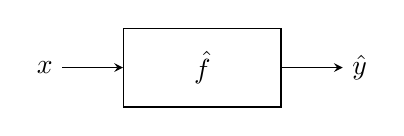
\begin{tikzpicture}
            \node (input) at (0, 0) [] {$x$};
            \node (output) at (4, 0) [] {$\hat{y}$};
            \node[rectangle, draw, minimum width=2cm, minimum height=1cm] (system) at (2, 0) {$\hat{f}$};
            \draw[-stealth] (input) -- (system);
            \draw[-stealth] (system) -- (output);
        \end{tikzpicture}
        \caption{Modelo del sistema.}
        \label{fig:system_model}
    \end{figure}

En primer lugar, para hallar $\hat{f}$, se debe definir el tipo de modelo a utilizar, es decir, la forma funcional de $\hat{f}$. Lo cual dependerá de la naturaleza del sistema a modelar. Existen dos principales clases de problemas de modelado: regresión y clasificación. La diferencia radica en el espacio de salida $y$. En los problemas de regresión, la variable de salida es continua, mientras que en los problemas de clasificación, la variable de salida es discreta y representa categorías o clases.

En segundo lugar, los parámetros $\theta$, para ajustar estos parámetros, se emplean técnicas de optimización que buscan minimizar la diferencia entre las salidas reales $y$ y las salidas estimadas $\hat{y}$ del modelo.

Tanto para la definición del modelo como para el ajuste de los parámetros, se depende en tener un conjunto de datos representativo del sistema a modelar, que contenga pares de entradas y salidas conocidas $(x_i, y_i)$. Es a partir de estos datos que se puede realizar un analisis de la relación entre las variables para definir la forma funcional del modelo $\hat{f}$ y luego, ajustar los parámetros para que el modelo se aproxime lo mejor posible al comportamiento del sistema real.

La definición de valores cuantitativos para evaluar que tan bien el modelo se ajusta al sistema real es fundamental para el proceso de validación del modelo. Estos valores se llaman métricas de evaluación y permiten cuantificar el desempeño del modelo en función de los objetivos específicos del mismo.
